
\chapter{Inleiding tot Complexiteitstheorie}

In Hoofdstuk~\ref{chap:talenautomaten} wordt bestudeerd of een gegeven
taal beslist/bepaald kan worden en welke machinerie daarvoor nodig
is. Als een taal beslist kan worden dan bestaat er een algoritme om de
beslissing (voo elke gegeven string) te nemen: een algoritme is
een voorschrift (of procedure of programma) dat altijd (t.t.z. voor
elke invoer) stopt. De natuurlijke vraag is dan: {\em hoe duur is het
  beslissingsproces}, en ook {\em hoe duur {\bf moet} het
  beslissingsproces zijn}.

Kost wordt altijd uitgedrukt in een aantal eenheden van een bepaald
type. In het geval van de uitvoering van een algoritme zijn er twee
natuurlijke types: tijd en plaats. In dit hoofdstuk gaat het
hoofdzakelijk over tijd. Tijd meten we gewoonlijk in veelvouden van
seconden of onderdelen ervan, maar die tijdseenheid is moeilijk te
formaliseren op een algemene manier: we willen de kost van een
algoritme of beslissingsprobleem niet laten afhangen van de toevallig
voorhanden technologie. Er is gelukkig een universele technologie,
namelijk de Turingmachine. Tijd betekent niks voor een TM, maar er
is wel de notie van een elementaire operatie in de TM: \'{e}\'{e}n
toepassing van $\delta$. Die gebruiken we als de tijdseenheid. Dit
model wordt later bekritiseerd, maar het zal overeind blijven. Om heel
precies te zijn: de TM heeft \'{e}\'{e}n band en die is onbeperkt in
beide richtingen; de lees/schrijfkop van de TM kan bij elke stap
naar links of naar rechts bewegen, maar ook stilstaan.

Om je inzicht te geven in de performantie van een algoritme zou je een
tabel kunnen krijgen met daarin voor een aantal invoerstrings $s$ de
tijd $time_A(s)$ die het algoritme $A$ nodig heeft om die string te
beslissen. Het is moeilijk om dat voor genoeg relevante strings te
doen en het is moeilijk om zulk een tabel goed te gebruiken of te
interpreteren. Het spel kan dus best op een andere manier gespeeld
worden, maar hoe? E\'{e}n ding is (bijna) zeker: we verwachten dat
het voor een langere string langer duurt om te beslissen of ie tot de
taal behoort. Daarom heeft het zin om de performantie van een
algoritme $A$ uit te drukken als een functie $time_A$ die de lengte
van de invoerstring afbeeldt op \'{e}\'{e}n van de volgende
grootheden:

\begin{verse}
- de minimale tijd die $A$ gebruikt om een string $s$ met $|s| = n$ te beslissen

- de gemiddelde tijd die $A$ gebruikt om een string $s$ met $|s| = n$ te beslissen

- de maximale tijd die $A$ gebruikt om een string $s$ met $|s| = n$ te beslissen
\end{verse}

\begin{sloppypar}
We zullen hier die laatste manier gebruiken. Ze staat bekend als de
{\em slechtste geval} {\mbox (tijds)complexiteit}: de formele
definitie komt later.
\end{sloppypar}

In dit hoofdstuk worden de volgende begrippen behandeld: 
\begin{verse}
- tijdscomplexiteit op een Turingmachine
\\
- de klasse \P en zijn robuustheid
\\
- certificaat en verifier
\\
- de twee definities van de klasse \NP
\\
- polynomiale reductie en $\N$P-compleetheid
\\
- voorbeelden van $\NP$-complete problemen: SAT, HAMPATH ...
\\
- de tijdshi\"erarchie
\\
- co-\NP en $\overline{\NP}$
\\
- een kijkje in ruimtecomplexiteit
\end{verse}




\section{Tijdscomplexiteit van algoritmen}
 
\grijs{\begin{definitie} Tijdscomplexiteit van een algoritme\\
{ De {\bf tijdscomplexiteit} van een algoritme $A$ is een functie
  $time_A(n):\N\rightarrow \N$ die voor een gegeven invoergrootte $n$
  het maximum aantal stappen aangeeft, die door het algoritme $A$
bij een invoeromvang van grootte $n$ worden gemaakt. Meer formeel:

~~~~~~~~~~~~~~~~~~~~$time_A(n) = max(\{time_A(s)|~|s| = n\})$ }

waarin $time_A(s)$ het aantal stappen is dat gemaakt wordt bij de
beslissing over $s$.
\end{definitie}}


Aan de definitie zien we dat $time_A(n)$ een {\bf slechtste geval}
maat is. Het is best mogelijk dat het algoritme voor de meeste strings
van lengte $n$ minder dan $time_A(n)$ stappen maakt en dat
slechts in enkele uitzonderlijke gevallen $time_A(n)$ stappen nodig
zijn.

Binnen complexiteitstheorie is het tijdsgedrag van een algoritme voor
grote invoer van belang. Bovendien is de echte tijdsduur van \'{e}\'{e}n
stap in de Turingmachine niet bepaald. Daarom is de
tijdscomplexiteit slechts op een constante na significant\footnote{Er
  is ook nog het linear speedup theorem!}. Dan is het volgende
handig:

\grijs{\begin{definitie} De (grote) $O$-notatie (In het Engels: ``big
    oh'')\\
{ Indien $f,g$ functies zijn van $\N$ naar
      $\R^+$, dan zeggen we ``$f(n)$ is $O(g(n))$'' (of $f$ is $O(g)$,
  en we schrijven ook $f(n)=O(g(n))$)
  indien
\[\exists c\in \R_0^+,\; \exists N\in \N,\;
\forall n\in \N: \; n\geq N \Rightarrow f(n)\leq c.g(n)\]

Men zegt: f is van orde g, of $f$ wordt asymptotisch gedomineerd door $g$.
}
\end{definitie}}

 

Het is mogelijk dat zowel $f$ is $O(g)$ als $g$ is $O(f)$.

\begin{vb}{
De functie die $n$ afbeeldt op $3n^2+4n +3$ is $O(n^2)$, omdat
\[ 3 n^2+4n +3 \leq 4 n^2,\;\; \forall n\geq 5 \;\;(c=4,\;\;N=5).\]
Omgekeerd is $n^2$ ook $O(3n^2+4n +3)$ omdat
\[ n^2 \leq 3 n^2+4n+3,\;\; \forall n\geq 0 \;\; (c=1,\;\; N=0). \]
}
\end{vb}

{\bf Zelf doen:} bewijs dat een positieve veelterm van graad $k$ 
$O(n^{k+i})$ is als $i \geq 0$ maar niet als $i < 0$; bewijs dat de
relatie {\em domineert asymptotisch} transitief is; geef twee functies
$f$ en $g$ zodanig dat $f$ is niet $O(g)$ en tegelijkertijd $g$ is
niet $O(f)$.



\grijs{\begin{definitie} Asymptotische equivalentie van functies.\\
{ Twee functies $f,g:\N\rightarrow \R^+$ worden asymptotisch
equivalent genoemd indien
\[ f\mbox{ is }O(g)\mbox{ en } g \mbox{ is } O(f) \]
We noteren deze situatie door $f$ is $\theta(g)$ (en dus
ook $g$ is $\theta(f)$).
}
\end{definitie}}



{\bf Zelf doen:} {\em asymptotisch equivalent} is een equivalentierelatie;
twee positieve veeltermen zijn asymptotisch equivalent als en slechts
als ze dezelfde graad hebben.



Met de $O$-notatie kunnen we algoritmen met elkaar
vergelijken. Veronderstel dat twee algoritmen $A$ en $B$ eenzelfde
probleem oplossen. We noteren de respectievelijke
complexiteitsfuncties met $time_A(n)$ en $time_B(n)$. Het algoritme
$A$ wordt beter (voor grote invoer) genoemd dan het algoritme $B$
indien

\begin{enumerate}
\item $time_A(n)$ is $O(time_B(n))$, maar
\item $time_B(n)$ is niet $O(time_A(n))$
\end{enumerate}
Indien we dus een algoritme $A$ hebben met een lineaire
tijdscomplexiteit
(t.t.z. $time_A(n)$ is $O(n)$)
en een algoritme $B$ hebben met een kwadratische
complexiteitsfunctie
($time_B(n)$ is $O(n^2)$),
dan beschouwen we $A$ als
een beter algoritme.
Nochtans mag men daarom niet besluiten dat algoritme $A$ altijd moet
verkozen worden boven $B$: de constante factor $c$ uit de definitie van
big oh, kan immers heel groot zijn voor $A$ en klein voor $B$ en
indien geweten is dat $n$ klein blijft, kan $B$ effici\"enter zijn.



Om goed te kunnen werken met dit begrip van complexiteit is het handig
om enkele functies en hun asymptotisch gedrag te kennen. In de rij
hieronder wordt van enkele belangrijke functies
hun asymptotisch gedrag gegeven: een functie $f(n)$ staat links van
$g(n)$ indien $f(n)$ is $O(g(n))$  (en niet omgekeerd).
\[ \log_2 n \;\; n\;\; (n\log_2 n)\;\;  n^2\;\; \cdots\;\; n^k\;\;
\cdots\;\; \;\;2^n \;\; n!  \]




\grijs{\begin{definitie}\label{TtimeTM} Gegeven een functie $T: \N
    \rightarrow \R^+$. We zeggen dat een Turingmachine $M$ loopt in
    tijd $T$ als $M$ op elke invoerstring $s$ stopt na hoogstens
    $T(|s|)$ stappen.
\end{definitie}}

Voor het gemak zeggen we dat $M$ een $T$-tijd Turingmachine
is. Het algoritme door $M$ bepaald is dan $O(T)$, maar niet omgekeerd.



\grijs{\begin{definitie} Een polynomiaal algoritme\\
{ Een algoritme is {\bf polynomiaal} (of polynoom) indien zijn
tijdscomplexiteit $O(n^k)$ is voor een $k\in \N$.}
\end{definitie}}

 



\grijs{\begin{definitie} Een exponenti\"eel algoritme\\
{ Een algoritme is {\bf exponenti\"eel} indien zijn
tijdscomplexiteit $\theta(c^n)$ is voor een re\"eel getal $c>1$.}
\end{definitie}}


Een kleine vergelijking toont aan dat algoritmen van exponenti\"ele
tijd heel wat minder effici\"ent zijn dan algoritmen van polynomiale
tijd. Veronderstel even dat een probleem kan opgelost worden door
middel van twee algoritmen $A$ en $B$, waarbij $A$ een
tijdscomplexiteit $time_A(n)=n^5$ heeft en waarbij
$time_B(n)=2^n$. Indien we deze algoritmen laten lopen op een machine
die 10 miljoen instructies per seconde kan uitvoeren, dan lost het
algoritme $A$ het probleem bij een probleemgrootte van $n=60$ in
minder dan 1,5 minuten op, terwijl het algoritme $B$ meer dan 3500
jaar nodig heeft! We zeggen dan {\em algoritme B schaalt slecht}.


We hebben er dus belang bij om voor specifieke problemen polynomiale
algoritmen te zoeken. Dat lukt niet altijd, en zelfs als het lukt is
het mogelijk dat de graad van de polynoom onpraktisch hoog is. Dan
moeten andere methoden gebruikt worden om aanvaardbare oplossingen
voor het probleem te construeren.



\paragraph{Wat als we andere machines gebruiken?}
Een heleboel andere berekeningsformalismen zijn ook
Turing-compleet. Dan lijkt het willekeurig om complexiteitstheorie op
te bouwen vanuit de TMs. We zien later waarom het toch werkt. Het is
bovendien mogelijk om de complexiteit van een algoritme uit te drukken
in het aantal elementaire operaties van een bepaalde soort
(bijvoorbeeld vergelijkinging van twee getallen, of omwisseling van
twee getallen): zo zegt men wel eens dat quicksort $O(n^2)$ is maar
die $n$ is het aantal te sorteren getallen, niet de
invoergrootte. Die $n^2$ telt het aantal vergelijkingen. Voor
quicksort is dat in het slechtste geval inderdaad $O(n^2)$, maar een
vergelijking op een TM kost vele stappen (en is afhankelijk van de
grootte van de voorstelling van de te vergelijken getallen). Bovendien
is {\em sorteren} geen beslissingsprobleem ...


\paragraph{Beslissen of berekenen?}

Beslissers gedragen zich als functies waarvan het bereik slechts twee
waarden heeft: accept en reject. Wat op de band van de TM staat, kan
ook beschouwd worden als het resultaat van een berekening. Dan
implementeert TM $M_f$ een functie $f$ met bereik $\Sigma^*$. Je kan
nu een TM $M_{fbit}$ construeren die als invoer een tuple $\langle s,i,b \rangle$ krijgt en
die accepteert als de $i$-de bit van $f(s)$ gelijk is aan $b$: $M_{fbit}$
gebruikt $M_f$ als {\em subroutine}. Zo zie je een sterk verband
tussen beslissen en berekenen. Ook omgekeerd werkt het: als je $M_{fbit}$
krijgt (zelfs zonder inwendig $M_f$) dan kan je $M_f$ bouwen, of toch
bijna ... Wat ontbreekt er nog?


\begin{sloppypar}
\paragraph{Niet-deterministische tijdscomplexiteitsklassen}
We hebben later ook nood aan een complexiteitsmaat voor
niet-deterministische Turingmachines (NDTM). Het niet-deterministisch
analoog voor Definitie~\ref{TtimeTM} is
\end{sloppypar}

\grijs{\begin{definitie}\label{TtimeNDTM} Gegeven een functie $T: \N
    \rightarrow \R^+$. We zeggen dat een niet-deterministische
    Turingmachine $M$ loopt in tijd $T$ als voor elke keuze van de
    overgang $M$ op elke invoerstring $s$ stopt na hoogstens $T(|s|)$
    stappen.
\end{definitie}}


\section{Tijdscomplexiteit van talen of beslissingsproblemen}


Nu we weten wat de tijdscomplexiteit van een algoritme is, kunnen we
proberen voor een gegeven taal $L$ het {\em beste} algoritme te
bepalen. Dat zou een karakterisatie geven van de moeilijkheid van een
beslissingsprobleem. Dat lukt echter niet. Een andere manier geeft wel
meer greep op de moeilijkheidsgraad van een probleem.

\subsection{Tijdscomplexiteitsklassen}



\grijs{\begin{definitie} DTIME(T)\\
{ DTIME(T) is de verzameling talen die beslist worden door een
  (deterministische) $c.T$-tijd Turingmachine, met $c > 0$.}
\end{definitie}}


$NDTIME(T)$ staat nu voor de talen die beslist kunnen worden door een
$c.T$-tijd NDTM.

{\bf Zelf doen:}
\begin{verse}
als $f = O(g)$, dan $DTIME(f) \subseteq DTIME(g)$.

$DTIME(T) \subseteq NDTIME(T)$
\end{verse}

De volgende definitie vat de klasse van talen die beslist kunnen
worden met een polynomiale Turingmachine:

\grijs{\begin{definitie} \P = $\cup_{k\geq 1} DTIME(n^k)$
\end{definitie}}

\paragraph{Voorbeelden van talen in \P}
\begin{itemize}
\item 
$Sum = \{\langle a,b,c \rangle| a,b,c \in \N \wedge a+b=c\}$
\item 
$Sorted = \{[a_1,a_2,...,a_n]| a_i \in \N \wedge (a_i \leq a_{i+1})\}$
\item 
$Connected = \{\langle G \rangle|G~is~een~samenhangende~graaf\}$
\end{itemize}

\paragraph{De definitie van \P is robuust.} 
We hebben vroeger vastgelegd dat de tijdscomplexiteitsfunctie wordt
bepaald op een Turingmachine met \'{e}\'{e}n lees/schrijf band, langs
twee kanten onbegrensd, en met de mogelijkheid om de leeskop te laten
stilstaan. Wat gebeurt met $\P$ als we een andere machine gebruiken?
Het antwoord is {\em niks} op voorwaarde dat we het normaal
houden: meerdere banden, een half-onbegrensde band ... het maakt niet
uit. We mogen zelfs random-access machines gebruiken,
meer-dimensionale banden ... Elk van die varianten kan met polynomiale
overhead gesimuleerd worden door de Turingmachines waartoe we ons
beperken. Het wordt gevaarlijk als we toelaten om in \'{e}\'{e}n cel
van het geheugen een willekeurig groot getal op te slaan, of op zulke
getallen rekenkundige operaties aan te rekenen met eenheidskost, maar
meestal is iets polynomiaal nog altijd polynomiaal. Het wordt
bijvoorbeeld raar als je de kost van de $n^{de}$ stap van de
Turingmachine een tijdskost $2^{-n}$ toekent\footnote{Zulk een machine
  heet een Zeno-machine.}: elk algoritme neemt nu hoogstens
\'{e}\'{e}n tijdseenheid ... en het is gedaan met
complexiteitstheorie.


\paragraph{En buiten \P ...} 
Voor sommige problemen volstaat polynomiaal veel tijd niet. Zo bestaat
een klasse van talen die exponentieel veel tijd vragen:

\grijs{\begin{definitie} \EXP = $\cup_{k\geq 1} DTIME(2^{n^k})$
\end{definitie}}

Het moet duidelijk zijn dat $\P \subseteq \EXP$. De inclusie is zelfs
strikt: zie Sectie~\ref{tijdshierarchie}.
%
Er bestaan ook beslisbare talen buiten \EXP: Presburger aritmetiek
levert een voorbeeld.

\paragraph{Wat met de encodering?}
Het wordt stilaan tijd om de encodering van de taal nader te
bekijken. Ons beslissingsprobleem is meestal geformuleerd zonder
direct naar een encodering te verwijzen. Zo kunnen we het hebben over
het probleem om te beslissen of een getal even is of oneven. Eens we
de codering vastleggen kunnen we aan een algoritme beginnen.

Er zijn zeker twee natuurlijke manieren om de natuurlijke getallen
te representeren: met een unair alfabet, en met een binair alfabet. In
de eerste heeft de voorstelling van $2048$ lengte 2048, in de tweede
heeft die lengte 12. We schrijven een $TM_u$ en een $TM_b$ voor elk van
die voorstellingen. De best mogelijke $TM_u$ moet tellen (modulo 2)
hoeveel tekens er in $s$ staan, en is dus $O(|s|)$. De beste $TM_b$
moet ook alle tekens van $s$ overslaan tot het laatste en neemt dan de
beslissing: weerom is het algoritme $O(|s|)$. Maar je ziet ook dat als
je de complexiteit uitdrukt in termen van de grootte van het getal dat
door $s$ wordt voorgesteld, de binaire representatie superieur is,
want voor $2048$ heeft $TM_b$ slechts iets meer dan $log_2(2048)$
stappen nodig, terwijl $TM_u$ er ongeveer 2048 nodig heeft. Langs de
ene kant geven beide encoderingen een lineaire complexiteit, langs de
andere kant heeft de unaire encodering exponentieel meer tijd nodig.

Een tweede voorbeeld maakt het nog erger: bekijk een na\"ief algoritme
om te bepalen of een getal $n$ priem is. Het bevat een lus van de vorm

\begin{algorithmic}
    \State{i := 2}
    \While {$i \leq n$}
         \If{i deelt n}
         \State{REJECT;}
         \EndIf
    \State{i += 1;}
    \EndWhile
    \State{ACCEPT}
\end{algorithmic}



In beide voorstellingen wordt de lus $n$ keer doorlopen, maar uitgedrukt
in de lengte van de representatie is dat met de binaire representatie
exponentieel meer dan met de unaire representatie. In het ene geval
zouden we kunnen denken dat het algoritme polynomiaal is, in het andere
geval is het exponentieel.

We moeten dus afspreken welke encodering we gebruiken om meer
eenduidig de complexiteit van een algoritme vast te leggen, en daarmee
samenhangend de complexiteitsklasse waartoe een taal behoort. Voor
getallen moeten we de binaire representatie gebruiken: een decimale
mag ook, maar niet de unaire. Voor andere objecten moeten we (soms
ad-hoc) afspreken welke de encodering is. Voor grafen bijvoorbeeld
gebruiken we de bits van de buurmatrix: alle redelijke representaties
zijn overigens naar mekaar omzetbaar met een polynomiale machine,
zodat de robuustheid van \P niet in het gedrang komt.

\subsection{De complexiteit van vermenigvuldigen: een korte uitstap}

Laten we voor het gemak een decimale voorstelling van getallen
gebruiken en even kijken naar het aantal elementaire
vermenigvuldigingen om twee getallen te vermenigvuldigen. Een
elementaire vermenigvuldiging is tussen twee getallen $\leq 9$: die
hebben constante kost. Voor het gemak bekijken we enkel het geval van
twee getallen met evenveel cijfers: $a = a_na_{n-1}...a_1$, en 
$b = b_nb_{n-1}...b_1$. We willen $a \times b$ berekenen. We leerden
op school een methode die $n^2$ elementaire vermenigvuldigingen doet,
en een hoop optellingen. Er werd lang gedacht - en zelfs als
conjecture geponeerd door A. Kolmogorov - dat het met minder niet
kon. A. Karatsuba liet zien dat het toch mogelijk is.

Veronderstel nu voor het gemak dat $n$ even is en gelijk aan $2m$. Dan
kan je $a$ en $b$ schrijven als
%
$a = A_{2}10^m + A_1$ en $b = B_{2}10^m + B_1$.
%
Dan is 

$~~~~~~~~~~a \times b = (A_{2}\times B_{2})10^{2m} + (A_{2}\times B_1 + A_1\times B_{2})10^m + A_1\times B_1 $ \\
waarin je 4 vermenigvuldigingen ziet.

A. Karatsuba merkte op dat de co\"effici\"ent van $10^m$ ook anders
berekend kan worden:

$~~~~~~~~~~(A_{2}\times B_1 + A_1\times B_{2}) = (A_{2} + A_1) \times (B_{2} +
B_1) - (A_{2}\times B_{2}) - (A_1\times B_1)$. \\
Daarin zijn de laatste twee vermenigvuldingen de co\"effici\"enten van
$10^{2m}$ en $10^0$. Door het resultaat van de laatste twee
vermenigvuldigingen te onthouden en te hergebruiken, is $a \times b$
te verkrijgen met slechts 3 vermenigvuldigingen. Door dit principe
recursief toe te passen (verdeel-en-heers) wordt vermenigvuldigen nu
$O(n^{log_2(3)})$. Ondertussen zijn algoritmen bekend met een lagere
complexiteit.

Wat leerden we uit dit uitstapje? Soms denken we intu\"itief dat iets
op slechts \'{e}\'{e}n manier mogelijk is, om dan later te ontdekken
dat er ook andere manieren mogelijk zijn.

\subsection{Certificaat en verifier}

De concepten certificaat en verifier worden hier ingevoerd los van
complexiteitsklassen.

\grijs{
\begin{definitie}\label{verifiercertificate}
Een {\bf verifier} voor een taal $L$ is een deterministische TM $V$
zodanig dat 

~~~~~~~~~~~~~~~~~~~~~~
$\forall s \in \Sigma^* : (s \in L \leftrightarrow \exists c \in \Sigma^*: V(\langle s,c \rangle) = accept)$


$c$ is een {\bf certificaat} voor $s$
\end{definitie}
}

In de context van complexiteitstheorie zullen we enkel {\em
beslissers} beschouwen, t.t.z. de $V$ in de definitie stopt op elke
invoer.


Wat voorbeelden:
\begin{itemize}
\item 
de taal $L$ is de verzameling van getallen die niet priem zijn; er
bestaat zeker een TM $M$ die samengestelde getallen accepteert, en de
priemgetallen reject, maar het is duidelijk dat als $s \in L$ dan
bestaat er voor die $s$ een certificaat $c$ - een deler - van dat
feit: de verifier $V$ moet dan enkel maar nagaan dat het certificaat
inderdaad die $s$ deelt; de taak van $V$ is eenvoudiger dan die van
$M$; merk op: je kan de verifier niet misleiden; of anders gezegd: als
ik de $V$ correct implementeer, dan kan geen enkel zogezegd
certificaat voor een gegeven $s$ mij ten onrechte doen geloven dat $s$
deelbaar is terwijl $s$ priem is

\item 
$L$ is de taal van tuples van de vorm $\langle G,a,b \rangle$ waarbij $G$ een graaf
is, en $a$ en $b$ knopen waartussen een pad bestaat in $G$; weerom
bestaat een TM $M$ die kan beslissen of een gegeven string tot $L$
behoort; een verifier $V$ voor die taal is eenvoudiger: het
certificaat kan een pad voorstellen van $a$ naar $b$; $V$ moet nu
enkel nakijken dat het certificaat echt een pad in $G$ is; $V$ heeft
minder werk dan $M$, want die moet een pad vinden - of op zijn minst
bewijzen dat er een pad bestaat; weerom is er geen manier om $V$ te
bedriegen

\item
$L$ is de taal van Turingmachines $M$ waarvoor $L_M$ niet leeg is;
deze taal is niet beslisbaar (dat zagen we vroeger); maar voor elke
Turingmachine $M$ met $L_M \neq \emptyset$ bestaat een certificaat,
namelijk een string $c \in L_M$ die een verifier kan gebruiken om te
laten zien dat die $c \in L_M$ 

\end{itemize}

De eerste twee voorbeelden geven de intu\"itie dat een verifier voor $L$
minder werk heeft (of kan hebben) dan een beslisser voor $L$. In het
derde voorbeeld is dat overweldigend duidelijk: er hoeft niet eens een
beslisser te bestaan, en toch bestaat een verifier en certificaat.

Confused? Denk na en lees Definitie~\ref{verifiercertificate} nog
eens na.

Het valt niet direct op, maar Definitie~\ref{verifiercertificate}
behandelt strings in $L$ anders dan strings in $\overline{L}$: er
bestaat een certificaat voor $s \in L$ maar voor $s \notin L$ is elke
string {\bf geen} certificaat.

De intu\"itie blijft overeind: een verifier heeft minder werk dan een
beslisser voor de taal. Er blijven vragen:
\begin{itemize}
\item 
heeft elke taal een verifier en een certificaat voor elke string in de
taal?
\item
kan er meer dan \'{e}\'{e}n certificaat bestaan voor een $s \in L$?
\item 
hoe moeilijk is het om het certificaat te construeren?
\end{itemize}

De tweede vraag heeft voor elke van de drie voorbeelden een {\em ja}
als antwoord: elke deler is een certificaat voor een deelbaar getal;
elk pad is een certificaat voor verbondenheid van $a$ en $b$; elke $s$
die in $L_M$ zit is een certificaat.

Als we die laatste vraag toetsen aan de drie voorbeelden, dan zien we
dat voor de eerste twee een certificaat kan gegeneerd worden: in het
eerste voorbeeld weten we niet of dat polynomiaal kan, in het tweede
geval wel. In het derde geval kan geen enkele altijd stoppende TM een
certificaat genereren voor elke invoer. Denk daarover toch even na,
want het is misschien subtieler dan je denkt.

Een bijkomende vraag over de lengte van het certificaat:
\begin{itemize}
\item 
is er een verband tussen de lengte van $s \in L$, de lengte van zijn
certificaat $c$, de moeilijkheid van het probleem?
\end{itemize}
Toets dit aan de drie voorbeelden.


Stel nu dat je weet dat als er een verifier $V$ en certificaat $c$
voor $s$ bestaan, en dat de lengte van $c$ begrensd is door een
functie $f$ van de lengte van $s$, dus:
%
$|c| \leq f(|s|)$. Nu kan je een certificaat genereren voor
%
$s \in L$, namelijk als volgt:

\begin{algorithmic}
    \ForAll {$(i \leq f(|s|) \wedge (c \in \Sigma^i)$}
         \If {$V(\langle s,c \rangle)$ accepts}
         \State{ACCEPT}
         \EndIf
    \EndFor
    \State{REJECT}
\end{algorithmic}

Dit algoritme loopt alle mogelijke certificaten op systematische
manier af. Het is een deterministisch algoritme. Wat kunnen we zeggen
over zijn complexiteit?

\begin{itemize}
\item 
de for-loop wordt $O(2^{f(|s|)})$ uitgevoerd in het slechtste geval
(we veronderstellen een alfabet met twee elementen)
\item 
als $V$ een $g$-tijd machine is, dan is de kost van de body van de for-loop
$O(g(|s|+|c|))$, dus $O(g(|s|+f(|s|)))$
\item
de totale complexiteit is $O(g(n+f(n))\times 2^{f(n)})$ met $n$ gelijk
aan de lengte van de invoer
\end{itemize}

Als $f$ minstens lineair is, dan is de complexiteit van dit algoritme
minstens exponentieel, zelfs als $g$ dat niet is. Je kan wel
argumenteren dat voor sommige problemen er een minder na\"ieve manier
bestaat om certificaten te genereren, minder na\"ief dan exhaustief,
maar het cruciale probleem is: voor heel wat problemen zijn {\em we}
daarin nog niet geslaagd. Dat wordt verder geformaliseerd in het
vervolg.

Het algoritme hierboven {\em raadt op systematische manier}. Die
systematiek kan gemodelleerd worden met een niet-deterministische
procedure waarbij de volgorde van de gegenereerde (potenti\"ele)
certificaten niet van belang is: een Prolog predicaat bijvoorbeeld.
Het kan ook gemodelleerd worden met een niet-deterministische Turing
machine {\em NDTM$_V$} waarbij er telkens twee mogelijkheden zijn voor de
overgang. Bij input $s$ schrijft {\em NDTM$_V$} in zijn eerste $f(|s|)$
stappen niet-determininstisch een string uit $\Sigma^{f(|s|)}$ op de
tape. Dan roept ie de deterministische verifier $V$ op. Als
\'{e}\'{e}n van de takken accpeteert, dan wordt $s$ geaccepteerd. 
Figuur~\ref{nondetverifier} illustreert dat: de lengte van het
certificaat is 2. 


\begin{figure}[h]
\begin{center}
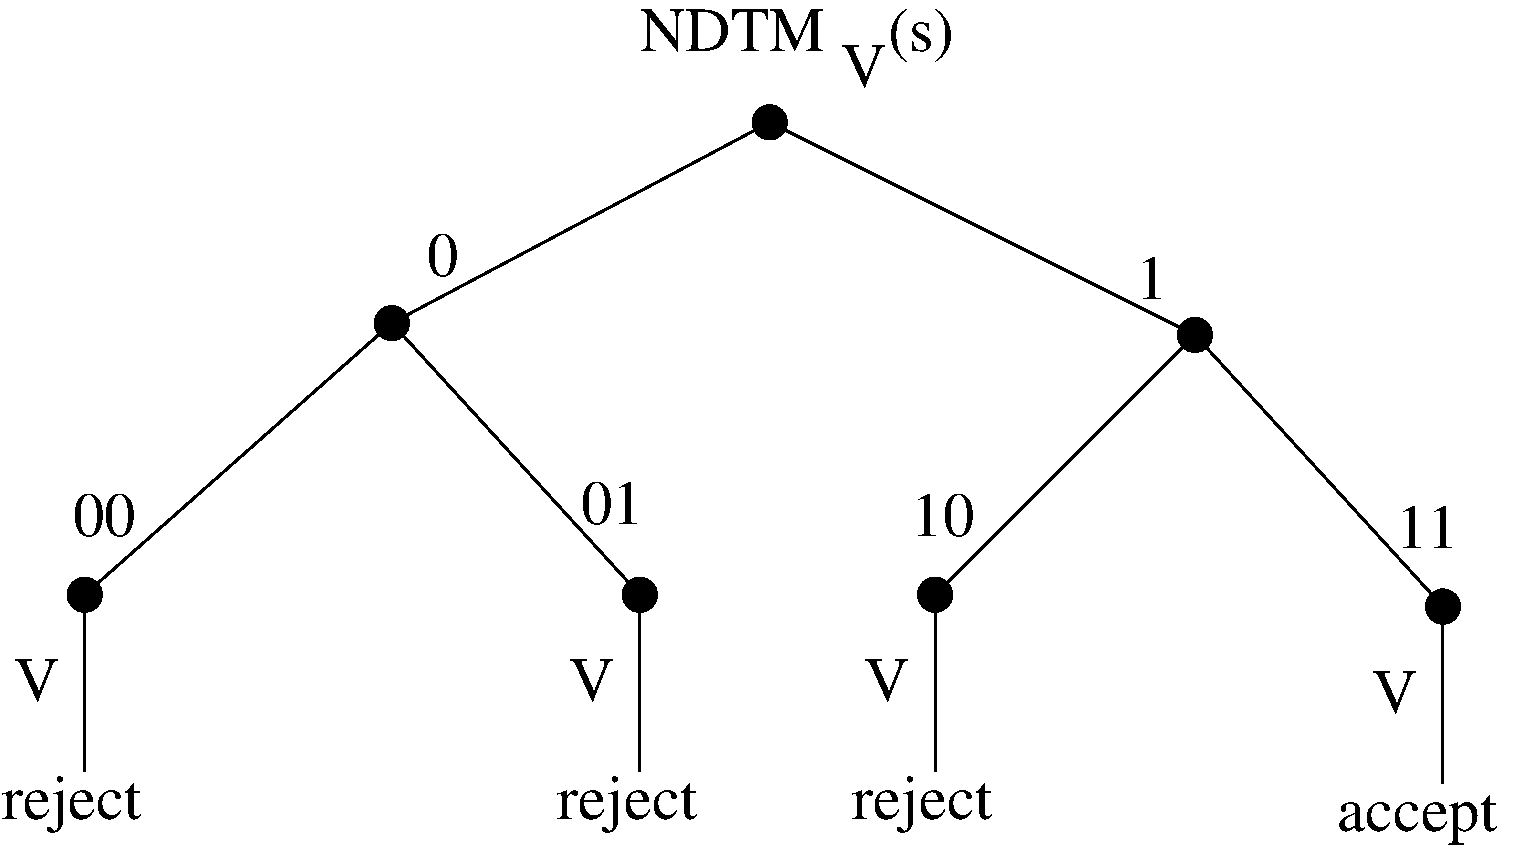
\includegraphics[height=0.2\textheight,keepaspectratio]{nondetverifier}
\caption{Generatie van het certificaat als de lengte gekend
is}\label{nondetverifier}
\end{center}
\end{figure}

Van die {\em NDTM$_V$} kunnen we nu opnieuw een verifier maken: die heeft
een certificaat nodig. Neem als certificaat een string die de keuzes
voorstelt die opeenvolgend gemaakt worden door {\em NDTM$_V$} om in een
accept-toestand te komen. Nu simuleren we de {\em NDTM$_V$} met die keuzes
met behulp van een deterministische machine ...

Daarmee is de zaak rond: van verifier+certificaat (met gekende lengte)
naar een niet-deterministische Turingmachine en terug.



\subsection{Twee definities van \NP}

De klasse \NP kan op twee manieren gedefinieerd worden.

\grijs{
\begin{definitie} Verifiers en \NP\\
\NP is de verzameling talen $L$ waarvoor een polynomiale verifier bestaat
en een polynoom $p$ zodanig dat een certificaat $c$ voor elke $s \in
L$ bestaat waarvoor $|c| \leq p(|s|)$.
~\\
~\\
Meer formeel: $L \in \NP$ als en slechts als

$~~~~~~~~\exists$ een polynomiale TM $M$ en een polynoom $p: \N \rightarrow \R^+$, zodanig dat

$~~~~~~~~~~~~~~~s \in L  \Leftrightarrow  \exists c \in \Sigma^{p(|s|)}$ met $M(\langle s,c \rangle) = accept$
\end{definitie}
}

De alternatieve definitie maakt gebruik van niet-determinisme.
\grijs{
\begin{definitie} Niet-determinisme en \NP\\
\NP is de verzameling talen $L$ geaccepteerd door een polynomiale
niet-deterministische Turingmachine.
\end{definitie}
}


De definities beschrijven dezelfde klasse van talen: het verband
tussen de twee definities is te vinden in voorgaande sectie. Je moet
nu kunnen argumenteren dat ook de definitie \NP robuust is t.o.v. het
uitvoeringsmodel.


Wat voorbeelden van talen in \NP:

\begin{itemize}
\item 
vermits $\P \subseteq \NP$ (zie je waarom?) kan elk probleem van \P
dienen als voorbeeld ...
\item 
koppels van isomorfe grafen (*)
\item 
de grafen met een Hamiltoniaanse kring (*)
\item
de niet-samenhangende grafen
\item
de gewogen grafen met tussen twee gegeven knopen een simpel pad dat
langer is dan een gegeven getal (*)
\item
verzin zelf iets!
\end{itemize}

Geef bij elk van de voorbeelden een beschrijving van een verifier en
het certificaat voor een gegeven string die tot de taal
behoort. Argumenteer telkens de polynomialiteit. Voor de voorbeelden
met een (*) is geen polynomiaal algoritme gekend.

{\bf Let op:} \NP staat voor {\em niet-deterministisch polynomiaal},
en niet voor {\em niet-polynomiaal}.

\subsection{Polynomiale reductie}

\begin{sloppypar}
We hebben vroeger talen gereduceerd naar andere talen: de many-one
reductie $\leq_m$ {\mbox bijvoorbeeld} (zie Pagina~\pageref{manyone}). Die
wordt hier wat verfijnd:
\end{sloppypar}

\grijs{\begin{definitie} Polynomiale reductie van een taal\\
{ Gegeven twee talen $L_1\subseteq \Sigma_1^*$ (op een
alfabet $T_1$) en $L_2\subseteq \Sigma_2^*$. We zeggen dat $L_1$
polynomiaal reduceert naar $L_2$ indien er een afbeelding
$f:\Sigma_1^* \rightarrow \Sigma_2^*$ bestaat waarvoor geldt:
\begin{verse}
1. $\forall x\in \Sigma_1^*$: \ \ \ $x\in L_1\Leftrightarrow f(x)\in
L_2$\\[2mm] 2. Er bestaat een (deterministische) TM die $f$ in
polynomiale tijd berekent.
\end{verse}
We noteren deze situatie door $L_1 \leq_p  L_2$.}
\end{definitie}}


$\leq_p$ verschilt van $\leq_m$ enkel in het feit dat de afbeelding
ook polynomiaal moet zijn en niet enkel maar berekenbaar door een TM.
$\leq_p$ is ook fijner dan $\leq_m$: als $A \leq_p B$ dan ook $A \leq_m B$.
Waren de voorbeelden van $\leq_m$ vroeger in de cursus soms ook $\leq_p$?



\grijs{\begin{stelling} \label{transitief}
De relatie $ \leq_p $ is transitief, of expliciet:
als $L_1 \leq_p L_2$ en $L_2 \leq_p L_3$ dan is ook $L_1 \leq_p L_3$.
\end{stelling}}
\begin{proof}   
Laat $f$ de polynomiaal berekenbare functie zijn die bij $L_1 \leq_p L_2$
hoort, en $g$ bij $L_2 \leq_p L_3$; $M_f$ en $M_g$ zijn de bijhorende
TMs: de ene is een $T_f$-machine, de andere een $T_g$-machine
waarbij $T_f$ en $T_g$ polynomen zijn. We bewijzen dat
%
$h = g\circ f$ de functie is die we zoeken voor $L_1 \leq_p L_3$.

Het is duidelijk dat $s \in L_1 \Leftrightarrow h(s) \in L_3$, en dat
$h$ berekenbaar is door een Turingmachine, namelijk de TM $M_h$ die
eerst $M_f$ laat lopen tot die klaar is, dan de leeskop helemaal naar
links verplaatst en dan $M_g$ laat lopen. We moeten dus enkel nog de
polynomialiteit van $M_h$ aantonen.

Laat $s$ met lengte groot genoeg de invoer zijn voor $M_h$. Op het
ogenblik dat $M_f$ klaar is, staat op de band een string $s_f$ van
lengte hoogstens $T_f(|s|)$. De leeskop naar links verplaatsen kost nu
hoogstens polynomiaal werk in $|s|$. Het uitvoeren van $M_g$ op $s_f$
neemt hoogstens $T_g(T_f(|s|)$ tijd, dus in het totaal hebben we als
bovenschatting van de totale tijd van $M_h$:
%
$T_f(|s|) + T_f(|s|) + (T_g \circ T_f)(|s|)$ hetgeen een polynoom is
in $|s|$.
\end{proof}


De volgende stelling lijkt een beetje op een stelling i.v.m. $\leq_m$.

\grijs{\begin{stelling}\label{P_is_klein}
Als $L_1  \leq_p  L_2$ en $L_2\in \P$ dan $L_1 \in \P$.
\end{stelling}}

\begin{proof}  Veronderstel dat $L_1\subseteq T_1^*$ en
$L_2\subseteq T_2^*$ en dat  $L_1 \leq_p  L_2$ via een afbeelding
$f:T_1^*\rightarrow T_2^*$ die in polynomiale tijd berekenbaar is
door een TM $M_f$. Omdat $L_2\in \P$ bestaat er een TM $M_2$ die $L_2$
beslist in polynomiale tijd. Construeer nu de TM $M$ die de TM $M_2$
na $M_f$ schakelt. We kunnen dan net zoals in het bewijs van de vorige
stelling aantonen dat $M$ een TM is met een polynomiale
tijdscomplexiteit.  Daarenboven is $M$ een TM die de taal $L_1$
beslist, dus geldt $L_1\in \P$.
\end{proof}



We beschouwen twee talen als equivalent indien de ene in de
andere polynomiaal gereduceerd kan worden en omgekeerd.



\grijs{\begin{definitie} Polynomiale equivalentie van talen\\
{
Twee talen $L_1$ en $L_2$ worden polynomiaal equivalent genoemd,
notatie $L_1\sim_p L_2$, indien
\[ L_1 \leq_p  L_2 \mbox{ \ en \ } L_2  \leq_p  L_1\]
}\end{definitie}}



De volgende eigenschap rechtvaardigt deze definitie.



\grijs{\begin{eig} De relatie $\sim_p$ is een equivalentierelatie.
\end{eig}}
\begin{proof}  We moeten  aantonen dat de relatie $\sim_p$
reflexief, symmetrisch en transitief is. De reflexiviteit volgt
onmiddellijk uit de definitie van een polynomiale reductie van  een
taal, waarin we voor $f$ de identieke functie kunnen nemen. Symmetrie volgt
onmiddellijk uit de definitie van $\sim_p$ en de transitiviteit werd  reeds
aangetoond in Stelling~\ref{transitief}.
\end{proof}



Zoals bij elke equivalentierelatie kunnen we ook hier de
equivalentieklassen beschouwen.  De klasse \P is opgebouwd uit drie
van deze equivalentieklassen.


\subsection{De klasse NP--compleet}

Binnen $\NP$ bestaat een speciale klasse talen: de moeilijkste van
$\NP$.

\grijs{
\begin{definitie}\label{defnpc} De klasse $\NP$--compleet\\
Een taal
$L$
is $\NP$--compleet als en slechts als
\begin{verse}
1. $L\in \NP$ en \\[2mm]
2. voor elke taal $L'\in\NP$ geldt dat $L' \leq_p  L$.
\end{verse}
De klasse van alle $\NP$--complete talen duiden we aan door $\NPC$.
\end{definitie}
}


Informeel kan je zeggen dat een
$\NP$--complete taal een taal is die zo moeilijk is dat elke andere
taal in $\NP$ er in polynomiale tijd naar kan vertaald worden. Of in
termen van problemen geformuleerd: een probleem is $\NP$--compleet als
het een oplossing heeft (in de vorm van een algoritme) zodanig dat elk
ander $\NP$ probleem een oplossing heeft die door een polynomiale
reductie van de $\NP$--complete af te leiden is. Het is helemaal
niet voor de hand liggend dat er $\NP$--complete talen bestaan, noch
of $\NPC$ niet samenvalt met $\NP$ of $\P$.  We illustreren echter
eerst hun belang aan de hand van de volgende stelling.

\grijs{\begin{stelling}$ $
\begin{verse}
1. \NPC is een equivalentieklasse voor de relatie $\sim_p$.\\[2mm]
2. Indien $\NPC\cap\P\neq \emptyset$ dan is $\NP=\P$.
\end{verse}
\end{stelling}}
\begin{proof} ~~
\begin{verse}
1. Veronderstel dat $L_1,L_2\in\NPC$. Dan geldt per definitie van
  $\NP$--com\-pleet\-heid dat zowel $L_1 \leq_p L_2$ als $L_2 \leq_p
  L_1$. Bijgevolg zijn $L_1$ en $L_2$ polynomiaal equivalent. De
  klasse $\NPC$ behoort dus tot \'e\'en enkele
  equivalentieklasse. Bovendien bestaan er geen elementen buiten
  $\NPC$ in deze equivalentieklasse, want indien $L\in\NP$ een taal is
  die equivalent is met een $\NP$--complete taal $L_1$, dan weten we
  dat voor elke andere taal $L'\in \NP$ geldt dat $L' \leq_p
  L_1$. Samen met $L_1 \leq_p L$, weten we dan dat
(Stelling~\ref{transitief}) $L' \leq_p L$, wat aantoont dat $L$ een
$\NP$--complete taal is. \\[2mm]
2. Stel dat $L\in\P \cap\NPC$. Beschouw een willekeurige andere taal
$L'\in \NP$. Omdat $L\in\NPC$ geldt dat $L' \leq_p L$. Hieruit en door
het feit dat $L\in\P$ volgt (door Stelling~\ref{P_is_klein}) dat ook
$L'\in \P$. Bijgevolg is $\NP=\P$.
\end{verse}
\end{proof}

De vorige stelling toont dus aan dat indien er \'e\'en $\NP$--compleet
probleem behoort tot de klasse van de problemen die oplosbaar zijn in
polynomiale tijd, alle problemen binnen de klasse \NP in polynomiale
tijd oplosbaar zijn. Alles wijst er echter op dat de klasse \NP niet
samenvalt met de klasse $\P$.\footnote{Hoewel ... Donald Knuth gelooft dat
$\P = \NP$.}

Figuur~\ref{NP-venn} toont de twee mogelijkheden: ofwel $\P \neq \NP$
ofwel $\P = \NP$.

\begin{figure}[ht]
\begin{center}
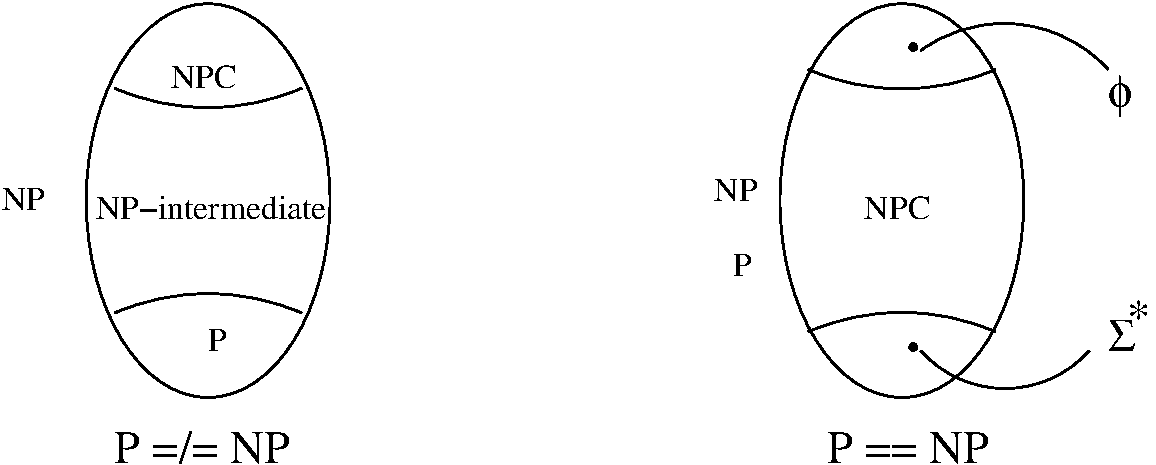
\includegraphics[width=0.7\linewidth,keepaspectratio]{NP-venn}
\end{center}
\caption{De (mogelijke) onderlinge ligging van de klassen $\P$, $\NP$
  en $\NPC$
 \label{NP-venn}}
\end{figure}
De verzameling $\NP$-intermediate is niet leeg in het geval dat $\P \neq
\NP$. Mogelijk is {\em isomorfe grafen} een element van \NP-intermediate.


Het eerste probleem waarvan men kon aantonen dat het tot \NPC behoort
was het {\bf vervulbaarheidsprobleem} (In het Engels: Satisfiability
Problem).  Dit probleem wordt vaak afgekort met de drie letters SAT en
we hebben eerst wat definities nodig: gegeven is een eindige
verzameling van booleaanse veranderlijken $U = \{u_1,u_2,\ldots,u_n\}$
(met andere woorden, elke veranderlijke $u_i$ kan de waarden ``waar''
of ``onwaar'' aannemen).  Met een atoom uit $U$ bedoelen we ofwel
\'e\'en van deze veranderlijken $u_i$ ofwel de ontkenning van \'e\'en
van deze veranderlijken die we noteren met $\neg {u}_i$ (te lezen als
{\em niet $u_i$}). Beschouw nu een formule in Conjunctieve NormaalVorm
(CNF) over $U$, t.t.z. een conjunctie van disjuncties van atomen,
zoals bijvoorbeeld
%
$C= (u_1 \vee u_2) \wedge (u_2 \vee \neg u_4 \vee u_7) \wedge  (\neg u_2 \vee u_3)$.

Het probleem is nu: gegeven een formule in DNF, bestaat er een
waarheidstoekenning aan de variabelen die de formule waar maakt.

Meer precies: SAT is de taal van formules in DNF die waar gemaakt
kunnen worden.

In 1971 kon Stephen A. Cook\footnote{Turing award 1982} de volgende stelling aantonen



\grijs{\begin{stelling} Stelling van Cook-Levin.
$SAT \in \NPC$
\end{stelling}}



Het bewijs van deze stelling valt buiten het bestek van deze
cursus. Inzien dat SAT behoort tot de klasse $\NP$ moet wel kunnen:
gebruik daarvoor eens de niet-deterministische definitie van $\NP$, en
ook eens de verifier-definitie. Hoe groot is het certificaat? Hoe heb
je de taal gecodeerd?

Eenmaal dit eerste $\NP$--compleet probleem bekend was, heeft men van
vele andere problemen ook kunnen aantonen dat ze $\NP$--compleet
zijn. Hier volgt een klein lijstje: grafen met Hamiltoniaanse kring,
grafen kleurbaar met een gegeven aantal kleuren, subgrafe-isomorfisme,
het knapzak probleem, pannenkoeksorteren, 0-1 integer programming,
heel wat combinatorische problemen en ook puzzels zoals Sudoku.

Als een taal $L$ enkel aan de tweede voorwaarde van Definitie
\ref{defnpc} voldoet, dan noemen we $L$ {\em NP-hard}. Men gebruikt de
term $\NP$--hard ook voor optimizatieproblemen waarvan de
beslissingstegenhanger $\NP$--compleet is. Er bestaan 
$\NP$--harde problemen die niet $\NP$--compleet zijn (m.a.w. niet in
\NP zitten): zo kan $SAT$ kan polynomiaal gereduceerd worden naar
$H_{TM}$, dus kan elk probleem in $\NP$ naar $H_{TM}$ gereduceerd
worden.


\subsection{Voorbeelden van polynomiale reducties}

\subsubsection{SAT naar 3-SAT}

3-SAT is zoals SAT, maar nu heeft in de DNF elke disjunctie exact 3
atomen. Hier is een formule uit 3-SAT:
%
$(a \vee b \vee \neg c) \wedge (\neg a \vee b \vee c)$. We laten zien
hoe een formule in DNF omgevormd kan worden tot dat formaat. Beschouw
elke disjunctie in de formule. Er zijn drie gevallen:
\begin{itemize}
\item 
de disjunctie bevat minder dan drie atomen: herhaal dan \'{e}\'{e}n van
de atomen tot er drie zijn;
\item 
de disjunctie bevat juist drie atomen: niets aan veranderen; of
\item 
de disjunctie bevat meer dan drie atomen: de disjunctie is van de vorm 
%
$a_1 \vee a_2 \vee  ... \vee a_n$ met $n > 3$.

Vind een nieuwe booleaanse veranderlijke uit, bijvoorbeeld $b$, en vervang
de disjunctie door twee disjuncties
\begin{verse}
(1) $b \vee a_{n-1} \vee a_n$ en

(2) $\neg b \vee a_1 \vee a_2 \vee  ... \vee a_{n-2}$
\end{verse}

Herhaal dat totdat geen enkele disjunctie langer is dan 3.
\end{itemize}

Controleer of deze transformatie
\begin{verse}
* een formule $\in SAT$ op een formule $ \in$ 3-SAT wordt afgebeeld

* een string $\notin SAT$ op een formule $ \notin$ 3-SAT wordt afgebeeld

* polynomiaal kan ge\"implementeerd worden op een TM 
\end{verse}

3-SAT $\in \NP$, want je kan voor elementen van 3-SAT een polynomiaal
certificaat geven. Alles samen levert dat op: 3-SAT zit in \NPC. Je
kan nu ook zien dat elke n-SAT met $n \geq 3$ ook $\NP$--compleet is.

\paragraph{2-SAT} is zoals 3-SAT, maar nu hebben alle disjuncties
exact twee atomen. Voor 2-SAT bestaan verschillende
polynomiale\footnote{in het aantal atoomvoorkomens} algoritmen - je
leest dikwijls zelfs lineaire algoritmen, maar dat is dan niet op een
TM, wel op een random access machine. In elk geval, 2-$SAT \notin \NPC$ ... of toch?


\subsubsection{3-SAT naar $k$-CLIQUE}

De taal $k$-CLIQUE bestaat uit tuples $\langle G,i \rangle$ waarbij $G$ een graaf is
met een clique van grootte $i$, t.t.z. $G$ bevat een subgraaf die
isomorf is met $K_i$. We tonen hoe de reductie werkt met twee
voorbeelden:

\begin{vb}
De formule is 
$(a \vee b \vee c) \wedge (a \vee \neg b \vee \neg c) \wedge (\neg a \vee b \vee \neg c) \wedge (\neg a \vee \neg b \vee c)$

\begin{figure}[h]
\begin{center}
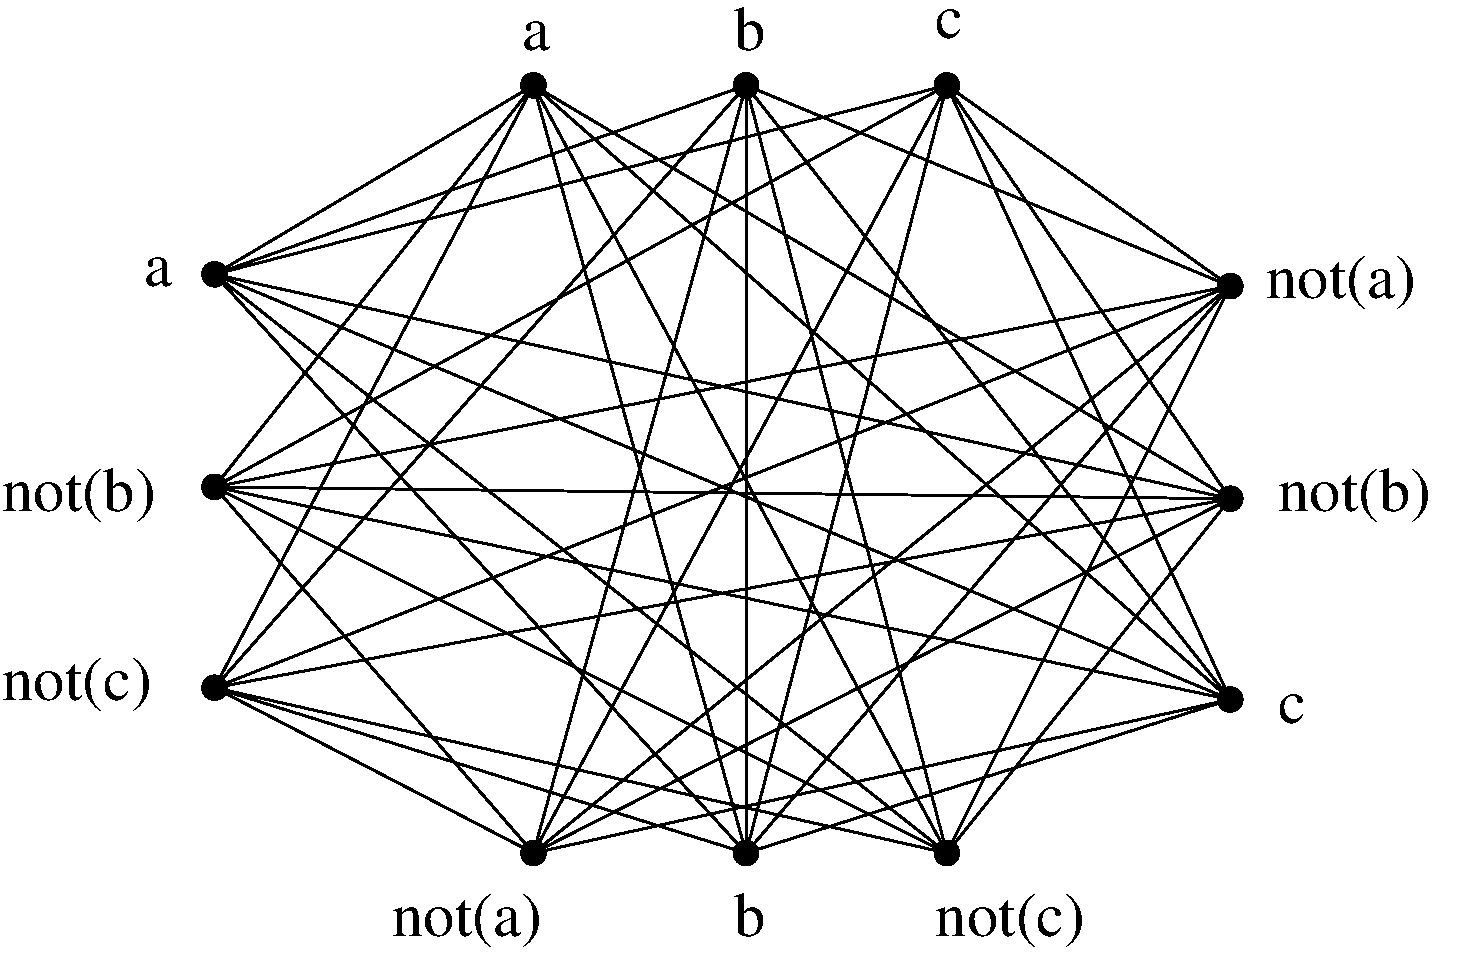
\includegraphics[height=0.2\textheight,keepaspectratio]{satclique}
~~~~~~~~~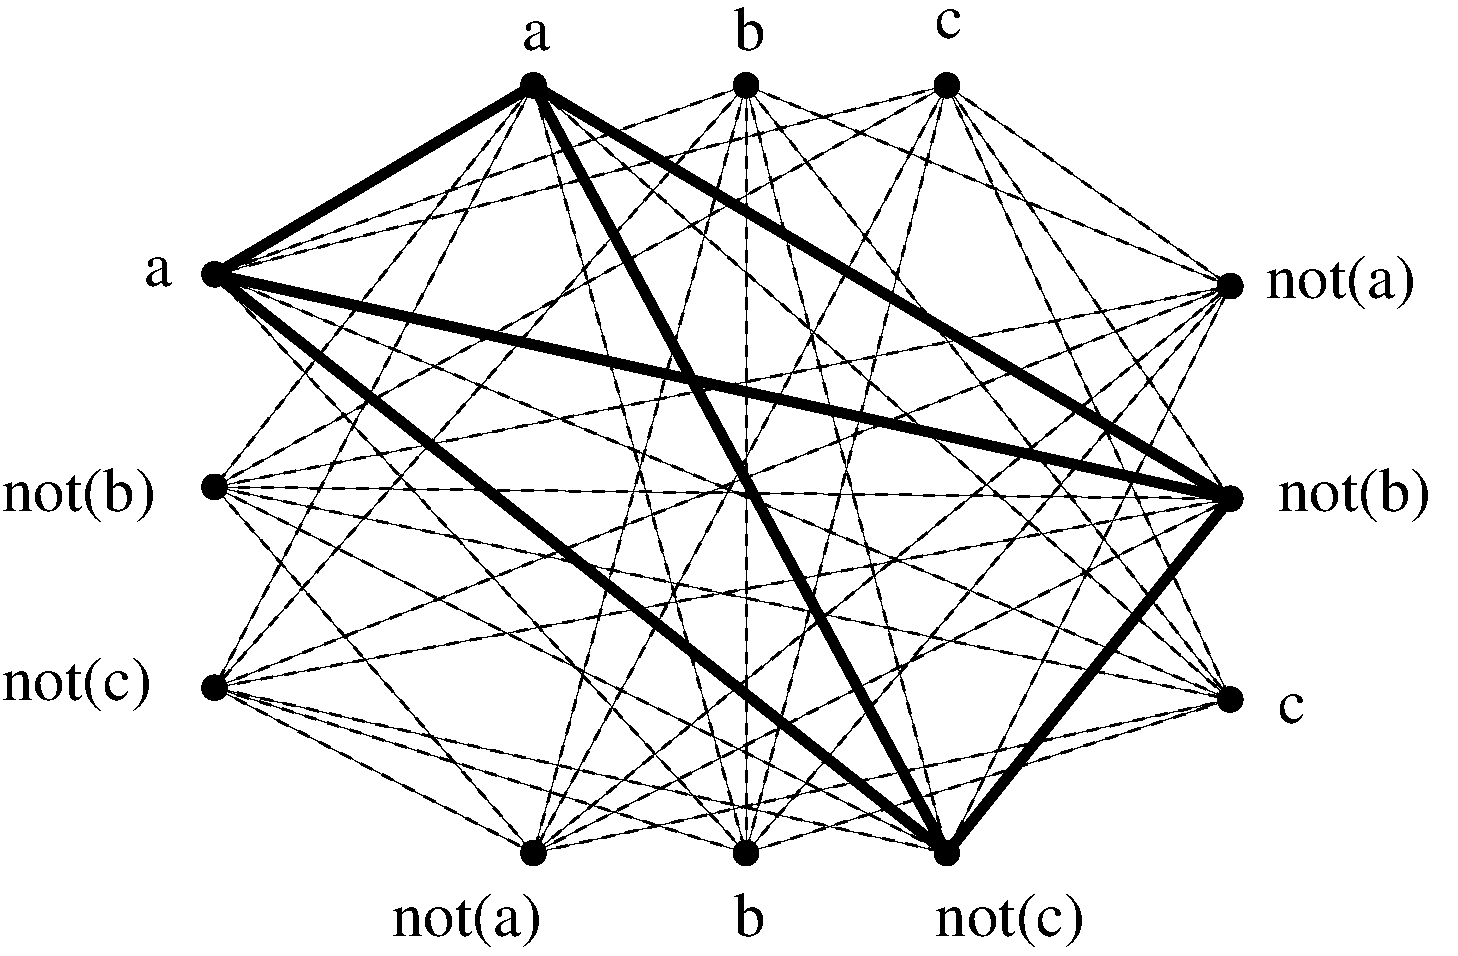
\includegraphics[height=0.2\textheight,keepaspectratio]{satcliquesol}
\caption{De graaf die overeenkomt met de eerste formule, en een 4-clique}\label{satclique}
\end{center}
\end{figure}

Figuur~\ref{satclique} toont links de graaf die de reductie oplevert:
\begin{verse}
- elk atoom correspondeert met \'{e}\'{e}n knoop met het atoom als naam

- een boog bestaat tussen twee knopen die {\em compatibel} zijn: $p$
en $\neg p$ zijn niet compatibel, en twee knopen die van dezelfde
disjunctie afkomstig zijn ook niet compatibel
\end{verse}

De buurmatrix van deze graaf kan je berekenen in polynomiale tijd. De
clique die je nodig hebt heeft als grootte het aantal disjuncties in
de formule.
\end{vb}

Je moet nog inzien dat de geproduceerde graaf een clique heeft van de
gevraagde grootte als en slechts als de formule behoort tot SAT.


\begin{vb}
We kunnen die reductie ook uitvoeren op kleinere disjuncties (je
mag eventueel atomen herhalen in een disjunctie). We nemen als formule
$(a \vee b) \wedge (\neg a \vee b) \wedge (a \vee \neg b) \wedge (\neg a \vee \neg b)$


\begin{figure}[h]
\begin{center}
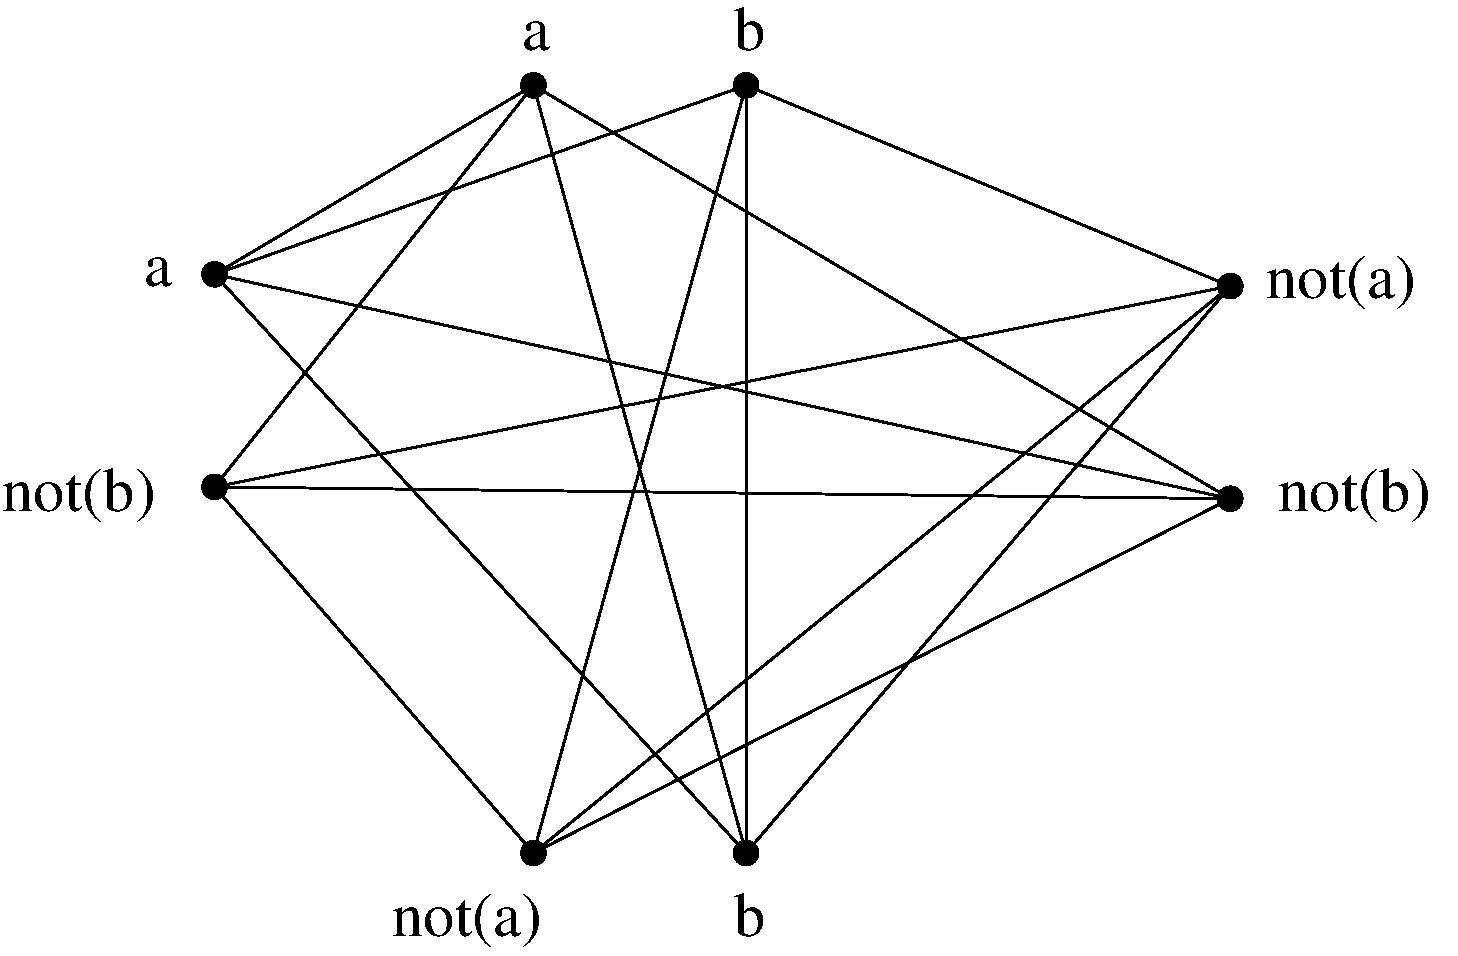
\includegraphics[height=0.2\textheight,keepaspectratio]{satclique2}
\caption{De graaf overeenkomend met de tweede formule: er is geen 4-clique}\label{satclique2}
\end{center}
\end{figure}

Omdat de graaf geen 4-clique heeft, behoort de formule niet tot
SAT. Er bestaan wel cliques in die graaf: de grootste $k$ waarvoor een
k-clique bestaat, geeft je het maximaal aantal disjuncties die je in
de formule tegelijkertijd kunnen waargemaakt worden. Zo zijn ook twee
optimizatieproblemen aan elkaar gelinkt.

\end{vb}

\newpage
{\bf Zelf doen:} 
\begin{verse}
- heb je een overeenkomst gezien tussen de SAT naar 3-SAT reductie en
de manier waarop een CFG in Chomsky-normaalvorm werd gezet?

- reduceer $3$-SAT naar SAT

- voorgaande was gemakkelijk omdat $3$-SAT $\subsetneq SAT$, daarom nog volgende vragen:

\begin{verse}
* als $A \subseteq B$ en $A \in \P$, dan ook $B \in \P$?

* als $A \subseteq B$ en $A \in \NP$, dan ook $B \in \NP$?

* als $A \subseteq B$ en $A \in \NPC$, dan ook $B \in \NPC$?

* als $A \subseteq B$ en $B \in \P$, dan ook $A \in \P$?

* als $A \subseteq B$ en $B \in \NP$, dan ook $A \in \NP$?

* als $A \subseteq B$ en $B \in \NPC$, dan ook $A \in \NPC$?

\end{verse}
\end{verse}


\subsection{Waarom zijn sommige problemen zo moeilijk?}

Voor SAT zouden we kunnen zeggen: er zijn $2^n$ mogelijke toekenningen
(met $n$ het aantal booleaanse variabelen), en onze intu\"itie zegt dat we
die allemaal moeten afgaan om een goeie te vinden ...

Voor Hamiltoniaanse kring zouden we kunnen zeggen: het aantal simpele
kringen in een graaf is exponentieel in het aantal knopen, en onze intu\"itie ...

Voor Minimaal Opspannende Boom zouden we kunnen zeggen: het aantal
opspannende bomen van een gegeven graaf met $n$ knopen kan $n^{n-2}$
zijn - dat is nog slechter dan exponentieel. Waarom hebben we
hierover niet diezelfde intu\"itie? Omdat een stelling uit de
grafentheorie ons een gulzig polynomiaal algoritme oplevert.

Misschien dat voor SAT de juiste stelling nog niet bewezen is, de
stelling die ons een polynomiaal algoritme oplevert, en dan kan onze
intu\"ite bijgesteld worden, net zoals toen Karatsuba het deed voor
vermenigvuldigen.

\section{De tijdshi\"erarchie}\label{tijdshierarchie}

Tot nu toe is de structuur van \P heel amorf. De
tijdshi\"erarchiestelling brengt daarin verandering: hieronder staat
niet de sterkste versie.

\grijs{
\begin{stelling} 
$DTIME(f) \subsetneq DTIME(f^2)$ voor elke $f$ die {\em
    time-constructible} is.
\end{stelling}
}

Ruwweg is een functie $f$ time-constructible als $f$ kan berekend
worden door een TM die $O(f)$ stappen nodig heeft en bovendien $f(n)
\geq n$. Mogelijk kom je van je leven nooit een functie tegen die
(niet triviaal) niet time-constructible is.

R. Stearns en J. Hartmanis bewezen in 1965 de eerste versie van de
tijdshierarchie, dus toch een aantal jaar voordat de notie van
$\NP$--compleet bestonden. O.a. daarvoor kregen ze (heel terecht) de
Turing award in 1993.

Los daarvan: het is belangrijk te beseffen dat je met $O(n^2)$ {\bf
  minder} kan doen dan met $O(n^4)$. Maar ook dat $O(4^n)$ meer kan
dan $O(2^n)$: tijd is een {\em resource} en wat je ermee kan doen is
beperkt. Overigens is dit een goed ogenblik om even na te denken over
\begin{verse}
- hoeveel talen zitten in $DTIME(n^k)$?

- hoeveel talen zitten in \P?

- hoeveel talen zitten in \NP?

- als je ergens {\em aftelbaar oneindig} antwoordde, is het dan ook opsombaar?
\end{verse}


\section{co-\NP}

Vermits de definitie van \NP elementen van de taal anders behandelt
dan elementen daarbuiten, heeft het zin om te onderzoeken of er iets
interessants te vertellen is over talen waarvan het complement in \NP
zit. Dat wordt gevat in

\grijs{
\begin{definitie} co-\NP: 
co-\NP = $\{L | \overline{L} \in \NP\}$
\end{definitie}
}

Pas op: co-\NP is niet gelijk aan $\overline{\NP}$. Het complement van
\NP bevat niet-beslisbare talen zoals $A_{TM}$, maar in co-\NP zitten
enkel beslisbare talen. Wat voorbeelden maken duidelijk dat het
helemaal niet evident is of co-\NP en \NP gelijk zijn.

\begin{verse}
- $SAT \in \NP$ want we hebben een kort (polynomiaal) certificaat voor
formules die satisfieerbaar zijn; $\overline{SAT} \in co$-$\NP$; hoe
zit het met certificaten voor $\overline{SAT}$? $\overline{SAT}$ bevat
formules die niet kunnen waargemaakt worden; welk kort certificaat zou
je daarvoor kunnen geven? niemand weet het

- langs de andere kant is er $TAUTOLOGY$, de taal van formules die
waar zijn voor {\bf elke} toekenning aan de variabelen;
$\overline{TAUTOLOGY}$ zit zeker in $\NP$: een kort certificaat bestaat
uit een toekenning die de formule onwaar maakt; maar een kort
certificaat dat kan geverifieerd worden zodat de formule inderdaad een
tautologie blijkt ... niemand kent het

- de gesorteerde rijen zitten in $\NP$; een certificaat voor een
niet-gesorteerde rij zou kunnen bestaan uit een index $i$ zodanig dat
het i-de element groter is dan het (i+1)-de; dus zit de taal van
gesorteerde rijen in co-$\NP$; je had natuurlijk kunnen zeggen: de taal
van gesorteerde rijen zit in $\P$, dus ook in co-$\NP$; juist, maar dan
had je iets gemist, namelijk het bedenken van een niet-triviaal en
polynomiaal certificaat

- COMPOSITE (de deelbare getallen) heeft een kort certificaat: een
deler van het gegeven getal; maar een kort certificaat voor PRIME is
moeilijk in te denken; langs de andere kant weten we sinds 2004 dat
PRIME $\in \P$, dus heb je niet eens een certificaat nodig
\end{verse}

Na deze voorbeelden moet je inzien dat $\P \subseteq \NP ~\cap$
co-\NP, en dat het helemaal niet duidelijk is of $\NP = $ co-\NP. \\
Ook moet je kunnen argumenteren dat als $\P = \NP$, dan $\NP = $
co-\NP. \\ Wat als $SAT \in$ co-$\NP$?

\section{$\NP$--compleet of $\P$?}

Hier willen we er alleen maar op wijzen hoe belangrijk de juiste
formulering van een probleem is. Beschouw de volgende twee talen:

\begin{verse}
- $k$-CLIQUE = $\{\langle G,i \rangle|$ i een geheel getal, G een graaf met een i-clique$\}$

- 7-CLIQUE = $\{\langle G \rangle|$ G een graaf met een 7-clique$\}$
\end{verse}

Van $k$-CLIQUE hebben we laten zien dat het in \NPC zit (we reduceerden
SAT ernaar), maar 7-CLIQUE is polynomiaal: stel $n$ het aantal knopen in G,
dan zijn er $C_n^7$ subsets van de knopen die mogelijk een clique vormen.
Nakijken of een bepaalde set van 7 knopen een clique vormt is
polynomiaal in de grootte van G, stel $O(n^c)$ voor een $c$. Vermits
$C_k^7 = O(n^7)$ hebben we een algoritme met complexiteit
$O(n^{c+7})$. Daar de encodering van G (als buurmatrix) zelf $O(n^2)$
is, zit het probleem in \P.

Bovenstaand fenomeen komt veel voor: \'{e}\'{e}n of meer parameters
van het probleem constant houden kan een polynomiale versie opleveren
van een $\NP$--compleet probleem.

Denk even terug aan de twee problemen:

\begin{verse}
- $A_{TM} = \{\langle M,w \rangle| w \in L_M\}$

- $E_{TM} = \{\langle M \rangle| \epsilon \in L_M\}$
\end{verse}

Door \'{e}\'{e}n parameter van $A_{TM}$ constant te houden krijgen we
$E_{TM}$. Levert dat iets op?



\section{Ruimtecomplexiteit}

Naast tijd is ook ruimte een resource: is je
Java-programma ooit al afgebroken omdat er niet genoeg plaats was voor
de runtime stack, of de heap? Of vertraagde de uitvoering van je
programma onaanvaardbaar wegens excessieve swapping of garbage
collection? Dan heb heb je het aan der lijve ondervonden. In eerste
instantie zou men ruimtecomplexiteit willen definieren als het aantal
cellen op de band die gelezen of geschreven worden. Dat is niet zo
nuttig omdat
\begin{verse}
- de invoer bij niet-triviale problemen helemaal gelezen moet worden,
dus ruimtecomplexiteit zou niet sublineair kunnen zijn: de ruimtekost
van de invoer is niet te vermijden

- anderzijds hebben veel algoritmen heel weinig {\bf extra} ruimte
nodig buiten de plaats van de invoer
\end{verse}

Dat laatste moet je bekend voorkomen: bv. om te testen of een rij
gesorteerd is, heb je enkel een index nodig in die rij en wat plaats
om de twee elementen die je wil vergelijken tijdelijk op te slaan; dat
is een kleine overhead (in termen van de grootte van de invoer).

Voor we aan de definities beginnen: ruimte kan je hergebruiken, tijd
niet. Daarom verwacht je dat {\em minder} ruimte dan tijd nodig is
voor een bepaalde taak.

Voor de definitie van ruimtecomplexiteit baseren we ons op een
TM-model met
\begin{verse}
- \'{e}\'{e}n read-only band met daarop de invoer

- \'{e}\'{e}n read-write band
\end{verse}
De ruimtekost van een algoritme wordt dan enkel bepaald door het
aantal cellen dat op de RW-band gebruikt wordt.


\grijs{
\begin{definitie}
DSPACE(f) is de verzameling talen die beslist worden door een
deterministische Turingmachine die $O(f)$ cellen op de RW-band
gebruikt.
\end{definitie}
}

\grijs{\begin{eig} \label{grootte_van_string}
Als de functie $f$ berekend wordt door een $T$-tijd TM, dan is
%
$|f(s)| \leq T(|s|)$.
\end{eig}}
Die eigenschap zegt essenti\"eel: de TM kan op niet meer vakjes van de
band schrijven dan dat hij stappen maakt.

Argumenteer dat $DTIME(f) \subseteq DSPACE(f)$. 


\grijs{
\begin{definitie}
$\PSPACE = \cup_{k\geq 1} DSPACE(n^k)$
\end{definitie}
}

Het is nu duidelijk dat $\P \subseteq \PSPACE$.

Voor ruimte is er een hierarchiestelling zoals voor tijd, dus o.a.
$DSPACE(f) \subsetneq DSPACE(f^2)$ voor {\em fatsoenlijke} $f$.

\grijs{
\begin{definitie}
$\NPSPACE$ is zoals \PSPACE, maar dan met niet-deterministische Turing
  Machines.
\end{definitie}
}

De inclusie $\PSPACE \subseteq \NPSPACE$ ligt voor de hand, en je zou
kunnen verwachten dat $\PSPACE$ niet gelijk is aan $\NPSPACE$, of dat het
niet geweten is. Hier dan toch een verrassing: $\PSPACE = \NPSPACE =$
co-$\PSPACE$. Dat niet-determinisme niks toevoegt aan $\PSPACE$ komt
weerom doordat ruimte herbruikbaar is: een niet-determininistische TM
kan met weinig ruimte-overhead deterministisch gesimuleerd worden. Dan
krijg je direct de intu\"itie dat ook co-$\NPSPACE$ gelijk moet zijn
aan $\NPSPACE$ en daaruit is de laatste gelijkheid af te leiden.

\paragraph{Minder dan lineaire ruimte?} Ook dat kan. Neem als
voorbeeld de taal van even getallen: die kan je beslissen door geen
extra ruimte te gebruiken. Dat werkt overigens voor alle reguliere
talen. Er zijn ook meer interessante talen die in sublineaire ruimte kunnen
beslist worden: neem het probleem van te beslissen of een gegeven
gerichte graaf $(V,E)$ een pad heeft tussen twee gegeven knopen. We
beschrijven een $log(n)^2$-ruimte algoritme, waarbij $n$ het aantal
knopen is in de graaf, in pseudo-code:

% \newpage
\begin{algorithmic}
\Function {existspath}{a,z,l}
\If {$(l = 0)$}
\State{return(a = z)}
\EndIf
\If {$(a,z) \in E$}
\State{return(TRUE)}
\EndIf


\ForAll {$(v \in V$}
   \If {{\sc existspath}$(a,v,l/2)~ \wedge~ ${\sc existspath}$(v,b,l-l/2)$}
   \State{return(TRUE)}
   \EndIf
\EndFor
\State{return(FALSE)}
\EndFunction
\end{algorithmic}

{\sc existspath}$(a,z,n)$ geeft TRUE terug als er een pad bestaat van a naar
z met lengte hoogstens l. Zijn tijdscomplexiteit is verschrikkelijk,
maar als je je inbeeldt dat dit op een klassieke machine wordt
uitgevoerd, dan merk je dat op de runtime stack nooit meer dan
$\log(n)$ stack frames nodig zijn, en dat elk stack frame in grootte
beperkt is tot $\log(n)$ bits. Het algoritme kan met dezelfde
ruimtecomplexiteit op een DTM ge\"implementeerd worden.

Verder is het interessant dat je ruimte en tijd kan uitwisselen: je
kan een versie van \mbox{{\sc existspath}} maken die minder tijd nodig heeft, maar
dan wel meer plaats gebruikt, bijvoorbeeld door een diepte-eerst
zoektocht in de graaf. Die heeft minder tijd nodig, maar je houdt dan
typisch in een knoop bij of je die al bezocht hebt: dat kost
\'{e}\'{e}n bit per knoop, dus lineair in het aantal knopen.

Log-ruimte gebruiken is interessant genoeg voor een eigen klasse:

\grijs{
\begin{definitie}
$\LL = DSPACE(\log)$
\end{definitie}
}

Log-ruimte algoritmen zijn belangrijk, bijvoorbeeld in de context van
grote databases of lange DNA-sequenties: met log van de plaats die een
database inneemt heb je genoeg plaats om pointers (binair) op te slaan
en te manipuleren. Met een constant aantal van die pointers heb je
dikwijls genoeg om de database te doorlopen, en queries te beantwoorden.

% \newpage
\section{Een rij van inclusies}

We hebben nu voldoende inzicht om een rij inclusies te verantwoorden:

\begin{verse}
$\LL \subseteq \NL \subseteq \P \subseteq \NP \subseteq \PSPACE = \NPSPACE \subseteq \EXP$
\end{verse}

Door de hierarchiestellingen weten we zeker dat $\LL \neq \PSPACE$ en
$\P \neq \EXP$, dus zijn sommige van die inclusies strikt, maar er is
niet bekend welke.


\section{Complexiteit en de Chomsky hi\"erarchie}

Is er een verband tussen de complexiteit waarmee een taal beslist kan
worden en zijn plaats in de Chomsky hi\"{e}rarchie?

Het is gemakkelijk in te zien dat een reguliere taal beslist wordt in
$O(n)$ stappen (van de FSA) met $n$ het aantal symbolen in de
input. Of dit ook kan in $O(n)$ stappen op een Turing machine valt nog
aan te tonen (door jullie). Je hebt ook heel weinig (extra) ruimte
nodig om een reguliere taal te beslissen: geen enkele. Met strikt
minder dan $\log$-SPACE kan overigens niks anders beslist worden dan
reguliere talen.

Voor context vrije talen is er een algemeen $O(n^3)$ (op een TM met 3
banden) algoritme: het algoritme van Cocke-Younger-Kasami. Het is een
vorm van {\em chart} of {\em tabular parsing}, of dynamisch
programmeren. Je komt ook toe met lineaire ruimte (de stapel), dus
$CFL \subset SPACE(n)$.

De niet-deterministische LBA beslist talen door niet meer plaats te
gebruiken dan de invoer: de context-sensitieve talen vormen dan ook de
klasse {\bf NSPACE}(n).


% \newpage
\section{Besluit}
Aan de basis van de studie\footnote{aanvang te situeren minstens 150
  jaar geleden!} van de complexiteit van algoritmen, ligt de wens om
binnen een bepaald formeel kader ``snelle'' algoritmen te
karakteriseren en de problemen die een ``snel'' algoritme
toelaten. Daarbij heeft men al vlug ingezien dat de grootte van de
input voor het algoritme een belangrijke rol moet spelen in die
karakterisatie.

Pas in 1965 werd door Jack Edmonds voorgesteld ``snel'' te
defini\"eren als ``polynomiaal in de lengte van de input'', daarmee
inspelend op het algemeen gevoel dat een polynomiaal algoritme snel
genoeg is en een exponentieel te traag. De problemen met een snelle
oplossing vormen $\P$. Problemen die niet in $\P$ zitten, worden
beschouwd als ``intractable'' of onbehandelbaar voor praktische
doeleinden.

Tegen het einde van de jaren 1960 werd het duidelijk dat voor sommige
ogenschijnlijk eenvoudige problemen (bijvoorbeeld SAT) niemand een
polynomiale oplossing vond. Steve Cook bedacht dan de notie van
``verifieerbaar in polynomiale tijd'', t.t.z. de problemen waarvoor in
polynomiale tijd kan geverifieerd worden of iets een oplossing is voor
het probleem en $\NP$ was geboren. In 1971 bewees Cook dan dat er
binnen $\NP$ een klasse problemen bestaat die het ``moeilijkst'' zijn,
nl. de klasse $\NP$-compleet en dat die klasse niet leeg is. Leonid
Levin (USSR) bewees hetzelfde resultaat onafhankelijk en praktisch
gelijktijdig, maar publiceerde natuurlijk in het Russisch en was
daarom minder bekend. Het sluitstuk is de realisatie dat indien
\'{e}\'{e}n probleem uit $\NP$-compleet ook in $\P$ zit, de twee
klassen $\P$ en $\NP$ samenvallen. De (on)gelijkheid van $\P$ en $\NP$
is echter nog steeds een open probleem, al lijkt wedden op gelijkheid
een slechte zaak: er zijn immers te veel problemen waarvoor heel wat
onderzoekers gezocht hebben naar een polynomiaal algoritme zonder het
te vinden.

Voorlopig is het onderscheid tussen $\NP$-compleet en $\P$ dus
belangrijk omdat men niet mag hopen op een effici\"ente
oplossingmethode voor intractable problemen (voor steeds grotere
invoer). Vermits heel wat alledaagse problemen $\NP$-compleet zijn
(vehicle routing, examenroosters opstellen ...) of een te hoge
exponent hebben (PRIME), werden andere oplossingsmethoden ontwikkeld,
samen met hun theorie. Zo bestaan er echt snelle probabilistische
methoden om na te kijken of een getal priem is (ze falen heel zelden),
en heuristieken en benaderingsschema's voor optimalisatieproblemen die
(nog) geen polynomiaal algoritme hebben. Soms kan een parameter van het
probleem gefixeerd worden, en dan krijgen we toch nog een tractable
probleem. Complexiteitstheorie heeft ook vertakkingen in cryptografie,
quantumcomputing, informatietheorie, circuit-design ... , maar de
centrale vraag blijft voorlopig of $\P = \NP$.

% \newpage
\section{Referenties}
\begin{itemize}
\item V.J. Rayward--Smith, ``Inleiding in de berekenbaarheidstheorie'',
Academic service, 1987
% \item S.A. Wiitala, ``Discrete Mathematics, a unified approach'',
% McGraw--Hill Book Company, 1987
% \item A.K. Dewdney, ``The Turing Omnibus, 61 Excursions in computer
% science'', Computer Science Press, 1989
% \item J.K. Truss, ``Discrete Mathematics for Computer Scientists'', 2nd edition, 
% Addison--Wesley, 1999
\item Sanjeev Arora and Boaz Barak, ``Computational Complexity: A Modern Approach'',
Cambridge University Press
\end{itemize}



